\subsubsection{PM2.5: Annual Context and a Source-Linked Case}\label{sec:pm25_case}
\begin{figure*}[t]
\centering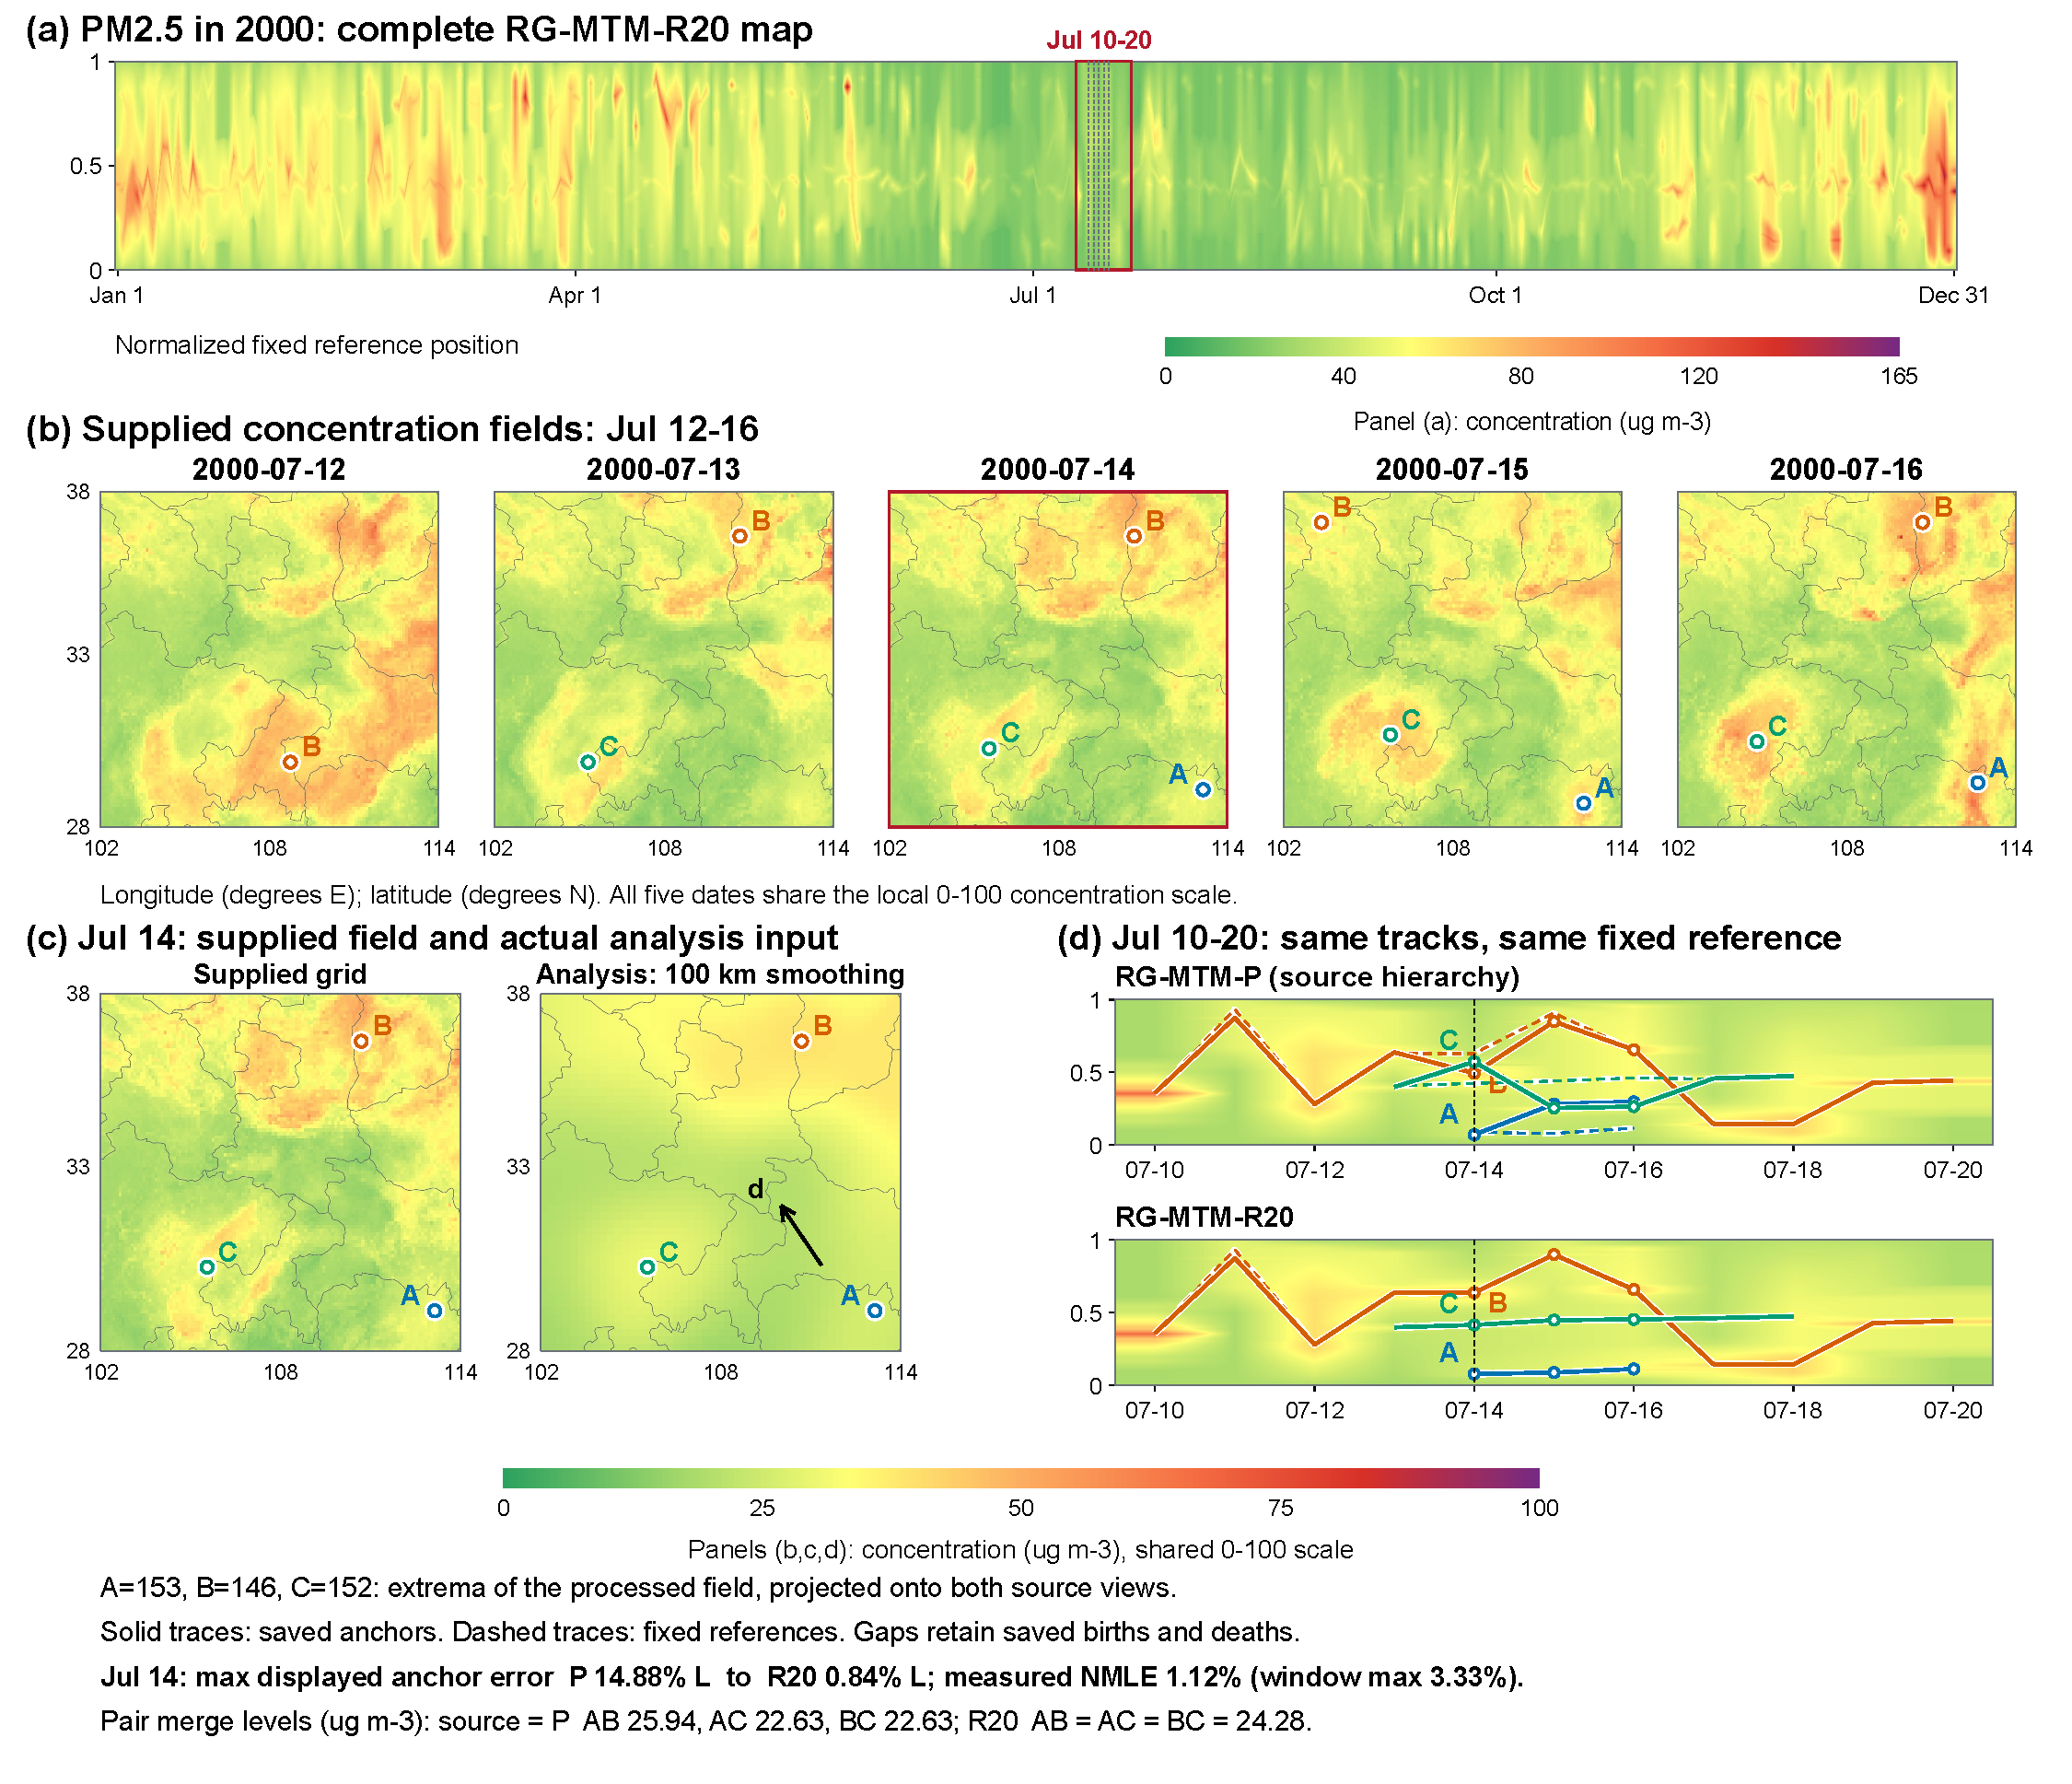
\includegraphics[width=\textwidth]{figures/Fig13.pdf}
\caption{PM2.5: complete-year context and a source-linked July case. (a) All 366 R20 profiles with July 10--20 outlined. (b) Supplied concentration fields for July 12--16, with geographic context from Natural Earth~\cite{NaturalEarth:Admin1}. (c) July 14 supplied and processed fields; markers show the same processed extrema $A=153,B=146,C=152$, and $d$ is the fixed annual reference direction. (d) Complete P/R20 profiles over July 10--20, with solid saved anchors and dashed fixed references. Tracks retain their saved births and deaths. Panel (a) uses 0--165\,$\mu$g\,m$^{-3}$; panels (b)--(d) share 0--100\,$\mu$g\,m$^{-3}$ without per-date rescaling. At July 14, maximum displayed-anchor displacement falls from 14.88\% to 0.84\% of $L$, at 1.12\% measured NMLE; the window's maximum NMLE is 3.33\%. This is a selected mechanism witness, not a claim of annual motion improvement. Display interpolation preserves every saved profile.}
\label{fig:pm25_case}
\end{figure*}

Figure~\ref{fig:pm25_case} connects the annual map to supplied concentration fields and the actual processed input. The geographic views retain the same 102--114\textdegree E, 28--38\textdegree N window; the analysis uses the existing $49\times49$ grid and fixed 100\,km smoothing and documented boundary treatment. The supplied grid and processed field are shown separately so that extracted extrema are not mistaken for independent observations or validated pollution objects.

For reproducible selection, we retain frames whose strongest three-feature interleaving witness exceeds $0.02L$ and whose three tracks coexist for at least three consecutive saved dates. Five of 34 witness frames satisfy the continuity condition. The frame closest to their median witness obstruction is July 14 (frame 195), with tracks $A=153,B=146,C=152$ continuing through July 16. Selection uses obstruction and continuity, rather than motion accuracy or achieved positional gain. Supplement S8 records the full candidate list and coordinate checks.

On July 14, the source hierarchy joins $A,B$ before $C$, while the fixed reference orders them $A,C,B$. P places $A,B,C$, and R20 uses $A,C,B$. From July 14 to 15, $C$'s reference increases by only $1.62\%L$, but its displayed P anchor decreases by $31.84\%L$ as the hierarchy-compatible arrangement changes. R20 increases by $3.27\%L$, following the reference direction. These are single-anchor changes, separate from the pairwise motion-error metric. The source views and dashed references distinguish a layout jump from a change in the processed extremum's projected position.

The positional gain has a measurable scalar price. On July 14, source/P connection levels are 25.9364\,$\mu$g\,m$^{-3}$ for $A/B$ and 22.6261\,$\mu$g\,m$^{-3}$ for either outside pair. R20 sets all three to 24.2813\,$\mu$g\,m$^{-3}$. The resulting worst-pair change is 1.6552\,$\mu$g\,m$^{-3}$, or 1.12\% of the fixed annual processed range; the local window reaches 3.33\% NMLE. This case explains a mechanism without overturning the annual comparison: P makes 42/95 motion errors and R20 makes 47/95. The tracked extrema do not establish pollutant transport, emission attribution, or the identity of a named haze episode.
